%\documentclass[preprint]{elsarticle}
\documentclass{jaac}
\usepackage[utf8]{inputenc}
\usepackage{amsmath}
\usepackage{amsfonts}
\usepackage{amssymb}
\usepackage{graphicx}
%\usepackage[authormarkup=none]{changes}
\usepackage[final]{changes}
%\usepackage[font=footnotesize]{caption}
%\usepackage{caption}
%\usepackage{subcaption}  % for subfigure
\usepackage{numprint} % round numbers
\usepackage{siunitx} % round numbers
\usepackage{booktabs}  % nice looking tables
\usepackage{indentfirst} % indent first line after section title
\usepackage{breqn} %break inline equation
\usepackage{tikz}
\usepackage{cases} %numcases and subnumcases
%\usepackage[symbol]{footmisc}
\usepackage[normalem]{ulem} %sout
\usepackage{textcomp} %texttildelow
%\usepackage{subcaption}

%%%%%%%%%%%%%%%%%%%%%%%%%%%%%%%%%%%%%%%%%%%%%%%%%%%%%%%%%%
%%%%%%%%%%%%%%%%%%%%%%%%%%%%%%%%%%%%%%%%%%%%%%%%%%%%%%%%%%
%JAAC
\def\currentvolume{*}
\def\currentissue{*}
\def\currentyear{*}
\def\currentmonth{*}
\def\doi{10.11948/\currentyear.\firstpage}
\firstpage{1}


\def\shorttitle{A Schwarz-based DDM for the dispersion eq.}


\def\shortauthor{J. G. Caldas Steinstraesser, R. Cienfuegos, J. D. Galaz Mora \& A. Rousseau}


\title{\uppercase{A Schwarz-based domain decomposition method for the dispersion equation}}

\author{Joao Guilherme Caldas Steinstraesser$^{1,\dag}$, Rodrigo Cienfuegos$^2$,  José Daniel Galaz Mora$^2$ and Antoine Rousseau$^3$}%%%%%%%%  Here is the full name of every author. %%%%%%%%%%%%%%%%%%

\date{}


\bibliographystyle{jaacbib}










%%%%%%%%%%%%%%%%%%%%%%%%%%%%%%%%%%%%%%%%%%%%%%%%%%%%%%%
%%%%%%%%%%%%%%%%%%%%%%%%%%%%%%%%%%%%%%%%%%%%%%%%%%%%%%%

\providecolor{added}{rgb}{0,0,1}
\providecolor{deleted}{rgb}{1,0,0}
%% Change tracking with ulem
%\renewcommand{\added}[1]{{\color{added}{}#1}}
%\renewcommand{\deleted}[1]{{\color{deleted}\sout{#1}}}

%\captionsetup{compatibility=false}
%\captionsetup[subfigure]{labelformat=parens,labelsep=space,font = scriptsize}

\renewcommand{\thefootnote}{\fnsymbol{footnote}}

\newcommand{\laplinv}{\mathcal{L}^{-1}}
\newcommand{\eF}{e^{-i \xi x }}

\renewcommand{\epsilon}{\varepsilon}


\definechangesauthor[color=orange]{2017}
\definechangesauthor[color=red]{1010}

\begin{document}





\baselineskip 12pt

\maketitle


\thispagestyle{first}\renewcommand{\thefootnote}{\fnsymbol{footnote}}
\footnotetext{\hspace*{-5mm}
\renewcommand{\arraystretch}{1}
\begin{tabular}{@{}r@{}p{10cm}@{}}
$^\dag$& the corresponding author. Email address:caldas-j@eleves.enpc.fr (J. G. Caldas Steinstraesser)\\
$^1$&MERIC, Marine Energy Research \& Innovation Center, Avda. Apoquindo 2827, Santiago, Chile\\
$^2$&Departamento de Ingeniería Hidráulica y Ambiental, Pontificia Universidad Católica de Chile, Av. Vicuña Mackenna 4680 - Macul, Santiago, Chile\\
$^3$&Inria and Inria Chile, Avda. Apoquindo 2827, Santiago, Chile\\
%$^*$& The authors were supported by National Natural Science
%Foundation of China (****) and National Science Foundation of
%Shanghai (*****).
\end{tabular}}

\vspace{-2mm}





\begin{abstract}
We propose \deleted[id=1010]{an optimized Schwarz Waveform Relaxation method} \added[id=1010]{a Schwarz-based domain decomposition method} for solving \added[id=2017]{a dispersion equation consisting on} the linearized KdV equation without the advective term, using simple interface operators based on the exact transparent boundary conditions for this equation. An optimization process is performed for obtaining the approximation that provides the method with the fastest convergence to the solution of the monodomain problem.
\end{abstract}

\begin{keyword}
Domain decomposition method, Schwarz method, transparent boundary conditions, KdV equation
\end{keyword}

\begin{MSC}
**, **.
(This is the 2010 Mathematics Subject Classification of your paper. Use comma ``," to separate each one.)
\end{MSC}


\section{Introduction}

\indent The Korteweg - de Vries (KdV) equation, derived by \cite{kdv1895} in 1895, models the propagation of waves with small amplitude and large wavelength, taking in account nonlinear and dispersive effects. In terms of dimensionless but unscaled variables, it can be written as \cite{BBM1971}

\begin{equation*}
	u_t + u_x + uu_x + u_{xxx} = 0
\end{equation*}

\indent As done in \cite{zheng2008} (and in \cite{besse2015} as a special case of their work), we will focus in this paper on the linearized KdV equation without the advective term : 

\begin{equation}
 \label{eq:DKdV}
	u_t  + u_{xxx} = 0
\end{equation}

\noindent to which we will refer as \emph{dispersion equation}.

\indent The work developed here is inspired from \cite{zheng2008} and \cite{besse2015}. Nevertheless, our objectives are different from theirs. In this paper we propose a domain decomposition method (DDM) for solving the dispersion equation \eqref{eq:DKdV} in a bounded domain, \emph{i.e.}, we will decompose the computational domain in subdomains and solve the problem in each one of them. Our work focuses in the formulation on appropriate and optimized conditions on the interface between the subdomains, in order to minimize the error due to the DDM and to accelerate the convergence of the method.

\indent The interface boundary conditions (IBCs) proposed here are simple approximations for the exact Transparent Boundary Conditions (TBCs) for the equation \eqref{eq:DKdV}, derived by \cite{zheng2008} and \cite{besse2015}. The TBCs make the approximate solution on the computational domain coincide with the solution of the whole domain, but its exact computation are not doable in general \cite{Xavieretal2008}. \cite{zheng2008} and \cite{besse2015} propose numerical approximations for these conditions, seeking to reduce the error created by the introduction of artificial boundaries.

\indent In the work presented here, we do not propose approximated transparent boundary conditions with the same objective (reducing the error related to the finitude of the computational domain). In fact, we intend to reduce the error created by the decomposition of the domain and the introduction of an artificial interface boundary condition, in the context of a DDM. In other words, we study the effectiveness of the boundary conditions as IBCs, not as TBCs. As a consequence, our work shall not use the same reference solution as the one used by \cite{zheng2008} and \cite{besse2015} : for validating their approaches, they compare their approximate solution with the exact solution in the whole domain. On the other hand, our reference solution will be the approximate solution computed on the computational monodomain.

\indent This paper is organized in the following way : in Section \ref{sec:TBC}, we recall the exact TBCs derived by \cite{zheng2008} for \eqref{eq:DKdV} and propose approximations for them, leading to very simple conditions (avoiding, for example, integrations in time) depending on two coefficients. With some numerical experiments, we show that these approximate TBCs work quite well (although not as well as the approaches of \cite{zheng2008} and \cite{besse2015}), motivating us to use them in the sequence of our work. In Section \ref{sec:DDM}, we describe the domain decomposition method used here and we construct it using our approximate TBCs as interface boundary conditions (IBCs). Small modifications are proposed for these IBCs such that the solution of the DDM problem converges exactly to the reference solution (the solution of the monodomain problem). Finally, we perform a large set of numerical tests in order to optimize the IBCs, in the sense that we search the coefficients for the approximate TBCs that provide the fastest convergence for the DDM iterative process.

\section{Application to a domain decomposition method}
\label{sec:DDM}

\indent The discrete approximations \eqref{eq:appDiscTBCP0} for the transparent boundary conditions for the equation \eqref{eq:DKdV} will be applied as interface boundary conditions (IBC) in a domain decomposition method (DDM). Firstly, following \cite{Japhet2003}, we will briefly describe the DDM that we will consider here, and after we will describe and test the incorporation of the proposed IBCs.

\subsection{The Schwarz Method}

\indent Domain Decomposition Methods allow to decompose a domain $\Omega$ in multiple subdomains $\Omega_i$ (that can possibly overlap) and solve the problem in each one of them. Therefore, one must find functions that satisfies the PDE in each subdomain and that match on the interfaces. 

\indent The first DDM developed was the Schwarz method \cite{Japhet2003,Gander2008}, which consists on an iterative method: in the case of a evolution problem, the solution  $u_i^{n,\infty}$, in each time step $t_n$ and each subdomain $\Omega_i$, is computed as the convergence of the solution obtained in each iteration, $u_i^{n,k}, \ \ k\geq 0$.

\indent We will consider here the Additive (or parallel) Schwarz method (ASM). In this method, the interface boundary conditions are always constructed using the solution $u_j^{n,k-1}, \ \ j \neq i$ of the previous iteration in the neighbor subdomains. Therefore, in each interface between the subdomains $\Omega_i$ and $\Omega_j$, the boundary condition for the problem in $\Omega_i$ is

\begin{equation}
	\label{eq:genericIBC}
\mathcal{B}_i(u_i^{n,k+1}) = \mathcal{B}_i(u_j^{n,k})
\end{equation}

\indent The ASM is a modification, proposed by \cite{Lions1988}, of the original (Alternating or Multiplicative) Schwarz Method, in which the IBCs are constructed using always the most updated solution of the neighbor domains. This modification originates an inherently parallel algorithm, which one naturally implements with parallel computing. The advantages obtained with the parallelism become more evident when the number of subdomains increases \cite{Lions1988}.

\indent In \eqref{eq:genericIBC}, $\mathcal{B}_i$ denotes the operator of the IBC. This operator allows the construction of of more general Schwarz methods : in the original one, the IBC's are Dirichlet conditions (\emph{i.e.}, $\mathcal{B}_i(u) = u$  ) \cite{Japhet2003,Lions1990}.

\indent Without loss of generality, in the following we will consider a domain $\Omega$ decomposed in two non-overlapping subdomains, $\Omega_1$ and $\Omega_2$, with $\Gamma = \Omega_1 \bigcap \Omega_2$.

\indent When implementing a Schwarz methods, one must define appropriate operators $\mathcal{B}_i$ such that :

\begin{itemize}
\begingroup \item There is a unique solution $u_i$ in each subdomain $\Omega_i$; \endgroup
\item The solution $u_i$ in each subdomain $\Omega_i$ converges to $u|_{\Omega_i}$, \emph{i.e.}, the solution $u$, restricted to $\Omega_i$, of the problem in the monodomain $\Omega$;
\end{itemize} 

\indent Moreover, one wants the method to show a fast convergence.

\indent In fact, accordingly to \cite{Japhet2003}, the optimal additive Schwarz method for solving the problem 

\begin{equation*}
\begin{cases}
\mathcal{A}(u) = f \ \ \text{in} \ \ \Omega\\
u = 0 \ \ \text{on} \ \ \partial\Omega\\
\end{cases}
\end{equation*}

\noindent where $\mathcal{A}$ is a partial differential operator, is the one which uses as interface boundary conditions the exact transparent boundary conditions, given by

$$B_i(u) = \frac{\partial}{\partial n_i}u + D2N(u)$$

\noindent where $\partial n_i$ is the outward normal to $\Omega_i$ on $\Gamma$ , and the D2N (Dirichlet to Neumann) operator is defined by

$$\left. D2N : \alpha(x) \mapsto \frac{\partial}{\partial n_i^c}v \right\rvert_\Gamma$$

\noindent with $\alpha$ defined on $\Gamma$. $v$ is solution of the following problem, solved in the complementary set of $\Omega_i$, denoted by $\Omega_i^c$

\begin{equation*}
\begin{cases}
\mathcal{A}(v) = f \ \ \text{in} \ \ \Omega_i^c\\
v = 0 \ \ \text{on} \ \ \partial \Omega_i \backslash \Gamma \\
v = \alpha \ \ \text{on} \ \ \Gamma
\end{cases}
\end{equation*}

\indent The ASM using such exact TBCs is optimal in the sense that it converges in two iterations, and no other ASM can converge faster \cite{Japhet2003}. Nevertheless, these TBC, in general, are not simple to compute both analtically and numerically. More specifically, they are nonlocal in time, so they must be approximated for an efficient numerical implementation \cite{Xavieretal2008}. It is in this context that we propose the implementation of our approximate TBCs as interface boundary conditions for the ASM.

\subsection{ASM with the approximate TBCs for the dispersion equation}

\indent The resolution of the dispersion equation \eqref{eq:DKdV} with the Additive Schwarz method, using the constant polynomial approximation for the TBCs, is written as

\begin{equation}
    \label{eq:problemDDM1}
    \begin{cases}
        (u_1^{n,k+1})_t + (u_1^{n,k+1})_{xxx} = 0 , \ \ x \in \Omega_1, \ \ t \geq t_0\\
        u_1^{n,0} = u_1^{n-1,\infty} , \ \ x \in \Omega_1 \\
        \Upsilon_1^{c_L}(u_1^{n+1,k+1},-L) = 0, \\ 
        \Theta_2^{c_R}(u_1^{n+1,k+1},0) = \Theta_2^{c_R}(u_2^{n,k},0) , \\
        \Theta_3^{c_R}(u_1^{n+1,k+1},0) = \Theta_3^{c_R}(u_2^{n,k},0)
     \end{cases}
\end{equation}

\begin{equation}
    \label{eq:problemDDM2}
    \begin{cases}
        (u_2^{n,k+1})_t + (u_2^{n,k+1})_{xxx} = 0 , \ \ x \in \Omega_2, \ \ t \geq t_0\\
        u_2^{n,0} = u_2^{n-1,\infty} , \ \ x \in \Omega_2 \\
        \Theta_1^{c_L}(u_2^{n+1,k+1},0) = \Theta_1^{c_L}(u_1^{n,k},0) \\
        \Upsilon_2^{c_R}(u_2^{n+1,k+1},L) = 0 \\
        \Upsilon_3^{c_R}(u_2^{n+1,k+1},L) = 0
     \end{cases}
\end{equation}

\noindent where $ \Upsilon_i, \ \ i=1,2,3$, are the external boundary conditions (\emph{i.e.}, defined on $\partial \Omega_i \backslash \Gamma$).

\indent Considering that we want to analyze and minimize the error due to the application of a domain decomposition method, the reference solution $u^{ref}$ in our study will be the solution of the monodomain problem

\begin{equation}
	\label{eq:problemMonodomain}
	\begin{cases}
	u_t + u_{xxx} = 0, \ \ x \in \Omega, \ \ t \in [t_0, t_0+\Delta t] \\
	u(t_0,x) = u^{exact}(t_0,x) , \ \ x \in \Omega \\ 
	\Upsilon_1(u,-L) = 0, \ \ t \in [t_0, t_0+\Delta t] \\
	\Upsilon_2(u,L) = 0, \ \ t \in [t_0, t_0+\Delta t] \\
	\Upsilon_3(u,L) = 0, \ \ t \in [t_0, t_0+\Delta t]
	\end{cases}
\end{equation}
	
\indent We notice that we will always compare the solutions computed along only one time step. This is necessary for the separated study of the DDM (without influence, for example, of the error accumulated along the time steps, due to the temporal discretization).

\indent The external BCs $ \Upsilon_i, \ \ i=1,2,3$ are independent of the interface BCs. Here, we will consider $\Upsilon_1 = \Theta_1^{c_L = 1.0}$, $\Upsilon_2 = \Theta_2^{c_R = 0.0}$ and $\Upsilon_3 = \Theta_3^{c_R = 0.0}$, which gives

\begin{equation*}
%	\label{eq:externalBCsDDM}
	\begin{gathered}
	\Upsilon_1(u,x) = u - u_x + u_{xx} = 0\\
	\Upsilon_2(u,x) = u = 0\\
	\Upsilon_3(u,x) = u_x = 0\\
	\end{gathered}
\end{equation*}

\indent This choice was made based on the easy implementation and the good results provided by the coefficients $c_L = 1.0$ and $c_R = 0.0$ in approximating the analytical solution in $\Omega$ (as shown in the table \ref{tab:firstTestsP0}). Nevertheless, it does not have much importance in the study that we will done here, as we want to study exclusively the behavior of the DDM. The only restriction for an appropriate study is that the external BCs for computing $u_{ref}$ must be the same $\Upsilon_i, \ \ i=1,2,3$, used for each subdomain in the DDM, as we did in \eqref{eq:problemDDM1}-\eqref{eq:problemDDM2} and \eqref{eq:problemMonodomain}.

\indent A simple analysis (for example in the Laplace domain) shows that the monodomain and DDM problems \eqref{eq:problemMonodomain} and \eqref{eq:problemDDM1}-\eqref{eq:problemDDM2} have an unique solution.

\paragraph{Remarks on the notation}

%\indent From here to the end of this paper, we will focus exclusively on the error produced by the DDM, compared to the referential solution, independently of the other possible components of the error compared to the analytical solution (external boundary conditions, error accumulation over the time steps, for example, as discussed in the introduction. 

\indent As the following study will be made considering the execution of the method over only one time step, we can suppress the index denoting the instant $t_n$ and use a clearer notation for the solution : $u_j^i$, where $i$ indicates the subdomain $\Omega_i$ (or, in the case of the reference solution, $i = ref$, and in the convergence of the method, $i = *$) and $j$ indicates the spatial discrete position. In the cases where the iterative process is taken into account, we will add the superscript $k$ to indicate the iteration.

\indent Concerning the spatial discretization, the monodomain $\Omega$ will be divided in $2N + 1$ homogeneously distributed points, numbered from $0$ to $2N$. In all the analytical description, we will consider that the two subdomains $\Omega_1$ and $\Omega_2$ have the same number of points, respectively $x_0,...,x_N$ and $x_N,...,x_{2N}$. The interface point $x_N$ is common to the two domains, having different computed solutions $u_N^1$ and $u_N^2$ in each one of them. Evidently, we expect, at the convergence of the ASM, that $u_N^1 = u_N^2 = u_N^*$

\subsection{Discretization of the problem}

\indent As done in the initial numerical tests in the section \ref{sec:TBC}, an implicit Finite Difference scheme will be used here. For the interior points of each one of the domains, we will consider a second order spatial discretization of the equation (\ref{eq:DKdV}):

\begin{equation}
    \label{eq:FDdiscretization}
    \frac{u_j^i - \alpha_j^i}{\Delta t} + \frac{-\frac{1}{2}u_{j-2}^i + u_{j-1}^i - u_{j+1}^i + \frac{1}{2}u_{j+2}^i }{\Delta x ^3} = 0
\end{equation}

\noindent which is valid for $j=2,...,N-2$ in the case $i=1$; for $j=N+2,...,2N-2$ in the case $i=2$; and for $j=2,...,2N-2$ in the case $i=ref$. In the above expression, $\alpha_j^i$ is a given data (for example, the converged solution in the previous time step).

\indent For the points near the boundaries, we use second order uncentered discretizations or an approximate TBC. Considering that one TBC is written for the left boundary and two for the right one, we have to impose an uncentered discretization only for the second leftmost point of the domain. For example, for the point $x_1$ : 

\begin{equation*}
    %\label{eq:uncenteredFDdiscretization0}
    \frac{u_{1}^2 - \alpha_{1}^2}{\Delta t} + \frac{-\frac{5}{2}u_{1}^2 + 9u_{2}^2 - 12 u_{3}^2 + 7\frac{1}{2}u_{4}^2 -\frac{3}{2}u_{5}^2}{\Delta x ^3} = 0
\end{equation*}

\noindent and similarly to the other points near the boundaries.

\indent In the resolution of the problem in $\Omega_1$, two interface boundary conditions are imposed (corresponding to $\Theta_2$ and $\Theta_3$) to the discrete equations for the points $x_{N-1}$ and $x_N$. On the other hand, in the resolution of the problem in $\Omega_2$, only one interface boundary condition is used (corresponding to $\Theta_1$), being imposed to the point $x_N$.

\paragraph{Remark : modification of the reference solution}

\indent  Even if the DDM with the proposed interface boundary conditions is compatible with the monodomain problem (which we will see that is not the case), the solution of the DDM does not converge exactly to $u^{ref}$, for a reason that does not depend on the expression of the IBCs, but on the fact that for each domain we write two boundary conditions in the left boundary and only one on the right. We are using a second order centered discretization for the third spatial derivative (which uses a stencil of two points in each side of the central point), implying that we must write an uncentered discretization for the point $x_{N+1}$ when solving the problem in $\Omega_2$. Therefore, this point does not satisfy the same discrete equation as in the reference problem. In order to avoid this incompatibility and allow us to study the behavior of the DDM, we will modify the discretization for the point $u_{N+1}$ in the monodomain problem, using the same second-order uncentered expression :

\begin{equation*}
    %\label{eq:uncenteredFDdiscretizationN}
    \frac{u_{N+1}^2 - \alpha_{N+1}^2}{\Delta t} + \frac{-\frac{5}{2}u_{N+1}^2 + 9u_{N+2}^2 - 12 u_{N+3}^2 + 7\frac{1}{2}u_{N+4}^2 -\frac{3}{2}u_{N+1}^2}{\Delta x ^3} = 0
\end{equation*}

\indent Figure \ref{fig:discretizations} resumes the discretizations imposed to each point in the monodomain and the DDM problems, as described above:

\indent 

\begingroup
\tikzstyle{label} =[above,font=\tiny]
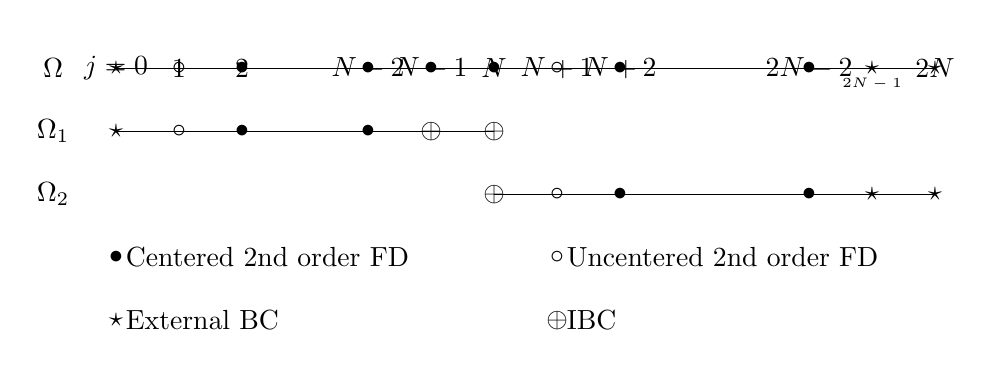
\begin{tikzpicture}[scale = .8]
	\coordinate (Alabel) at (-1,3);
	\coordinate (Aa) at (0,3);
	\coordinate (Ab) at (1,3);
	\coordinate (Ac) at (2,3);
	\coordinate (Ad) at (4,3);	
	\coordinate (Ae) at (5,3);	
	\coordinate (Af) at (6,3);	
	\coordinate (Ag) at (7,3);	
	\coordinate (Ah) at (8,3);	
	\coordinate (Ai) at (11,3);
	\coordinate (Aj) at (12,3);
	\coordinate (Ak) at (13,3);
	
	\draw (Aa) -- (Ak);
	\draw (Alabel) node {$\Omega$}; 
	\draw (Aa) node[label] {$j=0$};
	\draw (Ab) node[label] {$1$};
	\draw (Ac) node[label] {$2$};
	\draw (Ad) node[label] {$N-2$};
	\draw (Ae) node[label] {$N-1$};
	\draw (Af) node[label] {$N$};
	\draw (Ag) node[label] {$N+1$};
	\draw (Ah) node[label] {$N+2$};
	\draw (Ai) node[label] {$2N-2$};
	\draw (Aj) node[below,font=\tiny] {$2N-1$};
	\draw (Ak) node[label] {$2N$};
		
	\draw (Aa) node {$\star$};
	\draw (Ab) node {$\circ$};
	\draw (Aj) node {$\star$};
	\draw (Ak) node {$\star$};
	
	\draw (Ac) node{$\bullet$};
	\draw (Ad) node {$\bullet$};
	\draw (Ae) node {$\bullet$};
	\draw (Af) node{$\bullet$};	
	\draw (Ag) node{$\circ$};
	\draw (Ah) node {$\bullet$};
	\draw (Ai) node {$\bullet$};


	\coordinate (Blabel) at (-1,2);	
	\coordinate (Ba) at (0,2);
	\coordinate (Bb) at (1,2);
	\coordinate (Bc) at (2,2);
	\coordinate (Bd) at (4,2);	
	\coordinate (Be) at (5,2);	
	\coordinate (Bf) at (6,2);	

	\draw (Ba) -- (Bf); 
	
	\draw (Blabel) node {$\Omega_1$}; 
	\draw (Ba) node {$\star$};
	\draw (Bb) node {$\circ$};
	
	\draw (Bc) node {$\bullet$};
	\draw (Bd) node {$\bullet$};
	
	\draw (Be) node {$\oplus$};
	\draw (Bf) node {$\oplus$};	
	
	\coordinate (Clabel) at (-1,1);	
	\coordinate (Cf) at (6,1);	
	\coordinate (Cg) at (7,1);	
	\coordinate (Ch) at (8,1);	
	\coordinate (Ci) at (11,1);
	\coordinate (Cj) at (12,1);
	\coordinate (Ck) at (13,1);
		
	\draw (Cf) -- (Ck); 
	\draw (Clabel) node {$\Omega_2$}; 
	\draw (Cf) node{$\oplus$};
	\draw (Cg) node{$\circ$};
	\draw (Ch) node{$\bullet$};	
	\draw (Ci) node{$\bullet$};	
	\draw (Cj) node {$\star$};
	\draw (Ck) node{$\star$};
	
	%% Legend
	\draw (0,0) node {$\bullet$} node[right] {Centered 2nd order FD};
	\draw (7,0) node {$\circ$} node[right] {Uncentered 2nd order FD};
	\draw (0,-1) node {$\star$} node[right] {External BC};
    \draw (7,-1) node {$\oplus$} node[right] {IBC};
	
\end{tikzpicture}
\captionof{figure}{Scheme indicating the discretization imposed to each point in the monodomain and the DDM problems \label{fig:discretizations}}
\endgroup


\subsection{Corrections for the approximate IBCs}

\indent When using approximate TBCs in the ASM, one should guarantee that the converged solutions $u^*$ satisfy the same equation as the solution $u_{ref}$ of the monodomain problem. Nevertheless, one can easily see that, in the convergence, the solution $u^*$ does not satisfy the discrete equation \eqref{eq:FDdiscretization} on the points where the IBCs are imposed (the poins $x_{N-1},x_N \in \Omega_1$ and $x_N \in \Omega_2$). 

\indent As pointed out by \cite{Gander2001}, a finite difference discretization of the IBCs requires a special treatment to be consistent with the monodomain discretization. Therefore, we will formulate modified TBCs for the ASM in order to avoid this problem:

\begin{equation}
	\label{eq:correctedTBC}
    \begin{gathered}
        \Theta_1^{c_L}(u_2^{n+1,k+1}) + \theta_1 = \Theta_1^{c_L}(u_1^{n,k}) + \theta_1' \\
        \Theta_2^{c_R}(u_1^{n+1,k+1}) + \theta_2 = \Theta_2^{c_R}(u_2^{n,k}) + \theta_2' \\
        \Theta_3^{c_R}(u_1^{n+1,k+1}) + \theta_3 = \Theta_3^{c_R}(u_2^{n,k}) + \theta_3'
    \end{gathered}
\end{equation}

\noindent with $\theta_i, \theta_i'$ given by

\begin{gather*}
    \theta_1 = \Delta x c_L \frac{u_{N+1}^2 - 2u_{N}^2 + u_{N-1}^1}{\Delta x^2} + c_L^2\frac{\Delta x}{\Delta t} \left( u_{N}^2 - \alpha_{N}^2 \right)\\
    \theta_1' = - c_L^2\frac{\Delta x}{\Delta t} \left( u_{N}^1 - \alpha_{N}^1 \right)
\end{gather*}

\begin{equation*}
\begin{gathered}
    \theta_2 = \frac{\Delta x}{\Delta t} c_R^2 (u_N^1 - \alpha_N^1) \\
    \theta_2' = -\frac{\Delta x}{\Delta t} c_R^2 (u_N^2 - \alpha_N^2)
\end{gathered}
\end{equation*}

\begin{equation*}
\begin{gathered}
    \theta_3 = 2\frac{\Delta x}{\Delta t} \left[-\Delta x(u_{N-1}^1 - \alpha_{N-1}^1) - c_R (u_N^1 - \alpha_N^1) \right] + \Delta x \frac{u_{N-3}^1 - 2u_{N-2}^1 + u_{N-1}^1}{\Delta x^2} \\
    \theta_3' = 0
\end{gathered}
\end{equation*}

\indent It is straightforward to verify that the DDM problem with these modifications in the TBCs insure that the converged solution $u^*$ satisfies, in every point, the same discrete equations as the solution $u^{ref}$ of the monodomain problem \eqref{eq:problemMonodomain}.

\indent In addition, we notice that all the modification terms $\theta_i,\theta_i', \ i = 1,2,3$, are of order $O(\Delta x)$ (they are composed of discrete versions of time derivatives and second spatial derivatives multiplied by $\Delta x$). It is essential to insure that these terms are small, for the consistency with the approximate TBCs $\Theta_i$ to be fulfilled.

\subsection{Optimization of the IBCs (speed of convergence)}

\indent Our objective now is to optimize the IBCs in the sense of minimizing the number of iterations of the ASM until the convergence. We will make a very large set of tests in order to find the coefficients $c_L$ and $c_R$ (\emph{i.e.}, the constant polynomial approximation for the TBC) that provide the fastest convergence. To start with, we will make this study with fixed time step and space step, in order to analyze exclusively the influence of the coefficient.

\indent As we are interested in the speed with which the solution of the DDM method converges to the reference solution, the criteria of convergence used is

\begin{equation*}
%\label{eq:criteriaConvergence}
	e^{\Omega,k} \leq \epsilon
\end{equation*}

\noindent with $\epsilon = 10^{-9}$ and 

\begin{equation*}
	e^{\Omega,k} = ||u^{ref}_N - u^{k}_N||_2 = \sqrt{\Delta x \left[ \sum_{j=0}^N{(u^{ref}_j - u^{1,k}_j)^2 } + \sum_{j=N}^{2N}{(u^{ref}_j - u^{2,k}_j)^2 } \right] }
\end{equation*}
 
\indent In order to simplify the tests and avoid expensive computations, we will always consider $c_L = c_R = c$ in this optimization. The range of tested coefficients is $[-10.0, 20.0]$ (chosen after initial tests to identify a proper interval), with a step equal to  $0.1$ between them (or even smaller, up to $0.005$, in the regions near the optimal coefficients), and the maximal number of iterations is set to 100.

\subsubsection{Test varying the initial data and the interface position}

\indent As said above, in the first set of tests we will consider a fixed time step $\Delta t = 20/2560 = 0.0078125$ and a fixed mesh size $\Delta x = 12/500 = 0.024$. Moreover, we will consider two subsets of tests, that will allow us to study the speed of convergence with different initial conditions and different sizes of the subdomains:

\begin{enumerate}
	\item Tests varying the initial time step $t_0$, with the interface in the center of the monodomain $\Omega = [-6,6]$;
	\item Tests varying the position of the interface ($x_{interface} = -L + \alpha 2L$, where $L = 6$ and $0 < \alpha < 1$), for a fixed initial time $t_0 = 0.78125$.
\end{enumerate}

\indent In all the cases, the reference solution $u^{ref}$ will be the solution of the monodomain problem \eqref{eq:problemMonodomain}.

\indent The results are summarized in Figure \ref{fig:optimVarT0Interface}, with the number of iterations plotted as function of the coefficient $c$ (for the positive coefficients). We can see a very similar behavior of all the curves, with two minima whose position do not depend on $t_0$ and $\alpha$ (approximately, $c = 0.20$ and $c=4.5$). For $c<0$, the curves are very similar, with two minima located at $c = -0.10$ and $c = -1.35$, approximately. Moreover, the minima closest to zero ($c=-0.10$ and $c = 0.20$) are both associated with very discontinuous peaks, while the other two minima are associated with smoother curves. A detail of the curves around each positive minima are shown in Figures \ref{fig:optimVarT0PDetail} - \ref{fig:optimVarT0PDetail2} and \ref{fig:optimVarInterfacePDetail} - \ref{fig:optimVarInterfacePDetail2}. Finally, we remark that, for some curves, the minimal number of iterations is associated with the coefficients closest to zero, and, for other ones, to the other minimum, but the minimal number of iterations are very similar (between 5 and 7).

\begingroup
\addtocounter{figure}{1}
\noindent
\begin{minipage}[t]{.5\linewidth}
\begin{center}
	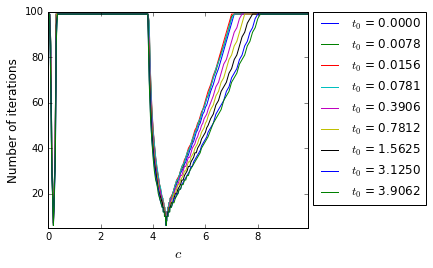
\includegraphics[scale=.375]{Fig3a.png}
	\captionof{subfigure}{General view (for a fixed interface and different values of $t_0$)}
\end{center}
\end{minipage}
\begin{minipage}[t]{.5\linewidth}
\begin{center}
	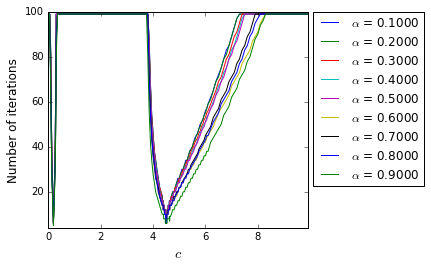
\includegraphics[scale=.375]{Fig3b.png}
	\captionof{subfigure}{General view (for a fixed $t_0$ and different positions of the interface)}
\end{center}
\end{minipage}
\begin{minipage}[t]{.5\linewidth}
\begin{center}
	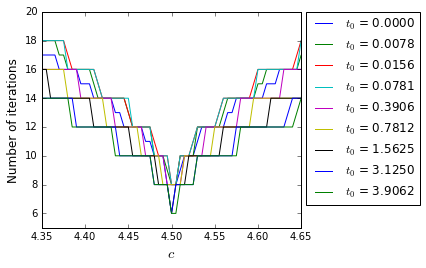
\includegraphics[scale=.375]{Fig3c.png}
	\captionof{subfigure}{Detail around one of the optimal coefficients (for a fixed interface and different values of $t_0$) \label{fig:optimVarT0PDetail} }
\end{center}
\end{minipage}
\begin{minipage}[t]{.5\linewidth}
\begin{center}
	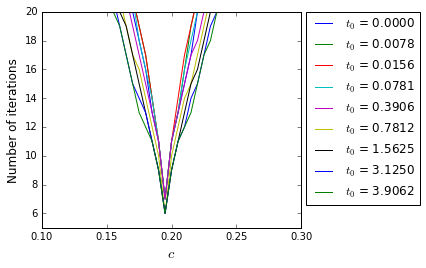
\includegraphics[scale=.375]{Fig3d.png}
	\captionof{subfigure}{Detail around the other optimal positive coefficient (for a fixed interface and different values of $t_0$) \label{fig:optimVarT0PDetail2}}
\end{center}
\end{minipage}
\begin{minipage}[t]{.5\linewidth}
\begin{center}
	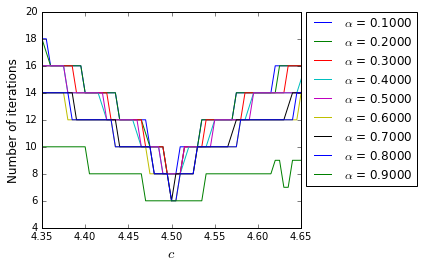
\includegraphics[scale=.375]{Fig3e.png}
	\captionof{subfigure}{Detail around one of the optimal coefficients (for a fixed $t_0$ and different positions of the interface) \label{fig:optimVarInterfacePDetail}  }
\end{center}
\end{minipage}
\begin{minipage}[t]{.5\linewidth}
\begin{center}
	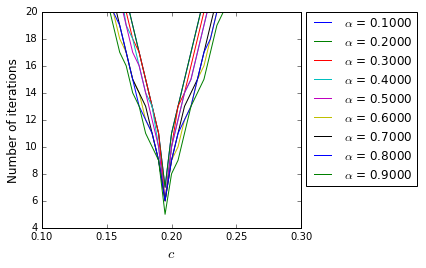
\includegraphics[scale=.375]{Fig3f.png}
	\captionof{subfigure}{Detail around the other optimal positive coefficient  (for a fixed $t_0$ and different positions of the interface) \label{fig:optimVarInterfacePDetail2}}
\end{center}
\end{minipage}
\addtocounter{figure}{-1}
	\captionof{figure}{Number of iterations until the convergence as function of the coefficient of the TBC, in the case of positive coefficients \label{fig:optimVarT0Interface}}
\endgroup

\indent Figure \ref{fig:errorEvolution} shows the evolution of the error, as function of the iterations, for the five positive coefficients $c$ that gave the fastest convergences, for a fixed initial instant and a fixed position of the interface. For other values of $t_0$ and $\alpha$ this graph is similar, concerning the number of iterations and the fact that the convergence is more regular for the coefficients closest to zero, compared to the other optimal coefficients.

\begingroup
\begin{center}
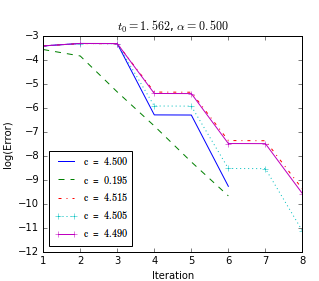
\includegraphics[scale=.5]{Fig4.png}
\captionof{figure}{Error evolution with the iterations for the fastest results \label{fig:errorEvolution}}
\end{center}
\endgroup

\subsubsection{Tests varying $\Delta t$ and $\Delta x$}

\indent After verifying that the method behaves similarly for every initial condition (\emph{i.e.}, every $t_0$) and every position of the interface, we will now keep these parameters fixed ($t_0 = 0$ and $\alpha = 0.5$) and make new tests with different values of $\Delta t$ (with fixed $\Delta x = 12/250$) and different values of $\Delta x$ (with fixed $\Delta t = 0.02$).

\indent The number of iterations as functions of the coefficient, for some of the tests, are shown in Figure \ref{fig:niterxCoefVarDtDx}, in the case of positive coefficients. The results for negative coefficients are similar.

\indent Figure \ref{fig:optimalCoefVarDxDtCorrectN} presents the optimal positive coefficient for each $\Delta t$ or $\Delta x$ (for one fixed value for the other coefficient). Considering the observation we did before about the similar results (\emph{i.e.} the number of iterations until the convergence) for the four optimal coefficients, we only took into account, for the construction of this curve, the positive minimum farther from zero: it was done because, as shown in Figure \ref{fig:niterxCoefVarDtDx}, these minima have a strong dependency on $\Delta t$ or $\Delta x$, and we will seek to study this relation.

\begingroup
\begin{minipage}{.5\linewidth}
\begin{center}
	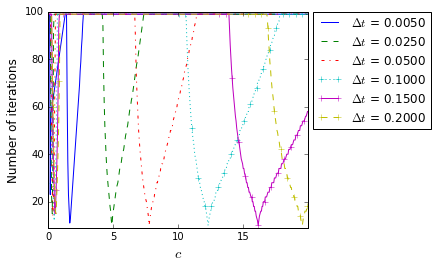
\includegraphics[scale=.375]{Fig5a.png}
\captionof{subfigure}{Fixed $\Delta x = \frac{12}{250}$}
\end{center}
\end{minipage}
\begin{minipage}{.5\linewidth}
\begin{center}
	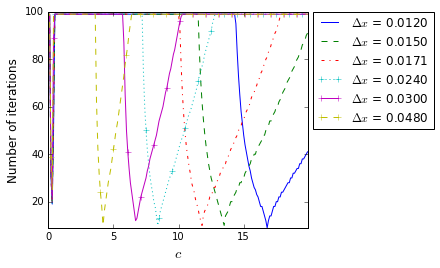
\includegraphics[scale=.375]{Fig5b.png}
\captionof{subfigure}{Fixed $\Delta t = 0.02$}
\end{center}
\end{minipage}
\captionof{figure}{Number of iterations until the convergence as function of the coefficient of the TBC (for positive coefficients)  \label{fig:niterxCoefVarDtDx}}
\endgroup


\begingroup
\begin{minipage}[t]{.5\linewidth}
	\includegraphics[scale=.4]{{Fig6a.png}}
	\captionof{subfigure}{Fixed $\Delta x = \frac{12}{250}$ }
\end{minipage}
\hfill
\begin{minipage}[t]{.5\linewidth}
	\includegraphics[scale=.4]{{Fig6b.png}}
	\captionof{subfigure}{Fixed $\Delta t = 0.02$ }
\end{minipage}
	\captionof{figure}{Optimal coefficients as function of the time step and the space step 	\label{fig:optimalCoefVarDxDtCorrectN}}
\endgroup

\indent Figure \ref{fig:optimalCoefVarDxDtCorrectN} suggests a dependence of the optimal coefficient on $(\Delta t)^\nu$ and $(\Delta x)^\eta$, with $0 \leq \nu \leq 1$ and $\eta < 0$. In fact, performing some regressions with $\Delta t $ or $\Delta x$ fixed, we could conclude that $\nu = \frac{2}{3}$ and $\eta = -1$ provide really well-fitted regression curves (with the coefficients of determination $R^2$ bigger than 0.99), both for the negative and the positive coefficients (although each one of these cases correspond to different curves). Therefore, we will seek to model a function

\begin{equation*}
	c_{opt}(\Delta t, \Delta x) = \kappa + \alpha (\Delta t)^{\frac{2}{3}} + \beta \frac{1}{\Delta x} + \gamma   \frac{(\Delta t)^{\frac{2}{3}}}{\Delta x}
\end{equation*}

\indent A regression using the corners of the rectangle $[0.001,0.1]\times[\frac{12}{100},\frac{12}{1000}]$ and fifteen inner points gives the surfaces

\begin{gather}
	c_{opt}^+(\Delta t, \Delta x) = 0.0775 -0.3353 (\Delta t)^{\frac{2}{3}} - 0.0012 \frac{1}{\Delta x} + 2.7407   \frac{(\Delta t)^{\frac{2}{3}}}{\Delta x} 	\label{eq:regression2DPos} \\
	c_{opt}^-(\Delta t, \Delta x) = -0.0583 -1.5024 (\Delta t)^{\frac{2}{3}} - 0.0006 \frac{1}{\Delta x} -0.7287  \frac{(\Delta t)^{\frac{2}{3}}}{\Delta x} 	\label{eq:regression2DNeg}
\end{gather}

\noindent respectively for the positive and the negative optimal coefficients. The coefficients of determination of each regression are $R^{2,+} = 0.9999894$ are $R^{2,-} = 0.9998993$, showing an excellent representation.

\indent In order to validate the expressions \eqref{eq:regression2DPos} and \eqref{eq:regression2DNeg}, we used them to compute the optimal coefficients for several points $(\Delta t, \Delta x)$, with $\Delta t \in [0.0005,0.3]$ and $\Delta x \in \left[ 12/5000,12/50\right]$. For almost all the points in the considered domain, the computed optimal coefficient provides a fast convergence to the monodomain solution, with less than 20 iterations, what is also observed in the case of the negative coefficients. The numbers of iterations observed are not always the smallest ones that we could find (cf. Figures \ref{fig:optimVarT0Interface} to \ref{fig:niterxCoefVarDtDx}), because the expressions \eqref{eq:regression2DPos} and \eqref{eq:regression2DNeg} are regressions constructed from optimal coefficients obtained among a discrete set of possible values. Nevertheless, they give a very good approximation for the optimal $c$ for each $(\Delta t, \Delta x)$, and one could search around a small region around the computed $c_{opt}$ to obtain an even faster convergence.

%\begingroup
%	\centering
%	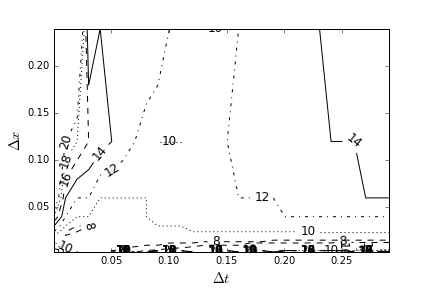
\includegraphics[scale=.6]{figures/FinalFigures/contourValidationP.png}
%\captionof{figure}{Contour lines showing the number of iterations until the convergence, when using the regressions surfaces for obtaining $c_{opt}^+(\Delta t, \Delta x)$ \label{fig:regressionValidation}}.
%\endgroup



\subsection{Partial conclusion}
 
\indent The results presented in this section show that the domain decomposition method proposed here, consisting in the additive Schwarz method with our approximate TBCs, is able to provide a fast convergence toward the solution of the monodomain problem. Furthermore, using the corrected TBCs \eqref{eq:correctedTBC}, this convergence is exact. Therefore, we reached our goals of solving the dispersion equation in a finite domain divided in two subdomains.

\indent Moreover, the results of the optimization tests are very satisfying regarding a more general application of our method. Firstly, for fixed spatial and temporal discretizations, we obtained optimal coefficients for the method independently of the initial solution and the size of the subdomains (\emph{i.e.}, independently of the initial instant and the position of the interface). Secondly, we obtained good regression expressions for the optimal coefficient as function of $\Delta t$ and $\Delta x$, which could allow the application of the model, with fast convergence, in other computational frameworks.














\section{Conclusion and outlook}

\indent We presented and implemented in this paper an \replaced[id=2017]{additive Schwarz method}{ optimized Schwarz Waveform Relaxation method} for the resolution of an one dimensional dispersive evolution equation, using as interface conditions between the subdomains some operators constructed based on the exact transparent boundary conditions for this equation. Although not as accurate (in the role of TBCs) as the ones proposed in the works we are based on (providing better TBCs was not our objective here), these approximate conditions stand out for its simple form and implementation and the fast convergence that they provide for the Schwarz method. Moreover, we also proposed small corrections to them, which insure that the solution of the DDM problem converges exactly to the solution of the monodomain problem. Finally, we verified that the speed of convergence depends on the time step, the mesh size and the (only) coefficient for constructing the approximate interface conditions; thus, via an optimization process, we obtained and validated regression expressions that provide the optimal coefficient (\emph{i.e.}, the one that provides the fastest convergence) in function of $\Delta t $ and $\Delta x$.

\indent \added[id = 1010]{Natural continuations of the work presented here would be the study of the method using more complex operators as IBCs, using for example higher-orders Padé approximations for $\lambda^2/s$ and considering different approximations for left and right boundary conditions. Moreover, we can extend this study for other problems, for instance the linearized KdV equation, which adds an advective term on the equation solved here, as well as other models of wave propagation. Finally, we can seek the development of global in time Schwarz methods, using optimized Scwharz waveform relaxation methods.}
\begin{acknowledgements}

\indent This study was conducted under the Marine Energy Research \& Innovation Center (MERIC) project CORFO 14CEI2-28228, and thanks to the support of international partnerships department of Inria, through fundación Inria Chile.

\indent The authors also want to thank Philippe Bonneton and Véronique Martin for fruitful discussions related to this work.

\end{acknowledgements}

\bibliography{biblioPaper}
\newpage
\end{document}
